\chapter{\label{ax:c-the_score_in_live_electronics_music}Case Study. The score in Live Electronics Music}

Throughout this research project, multiple case studies were conducted to examine the types of documentation found in live electronic music scores. We focused on the instruction formats and lexicon used to document technologies, setups, and staging in compositions that adopt unconventional or ``anti-academic'' approaches, which require extensive prior understanding before performance.\\
From the late 20th century onward, the traditional musical score has significantly expanded. Pursuing new sounds and advanced instrumental techniques has required new symbols and instructions that extend beyond conventional musical notation. The post-war arrival of electronics in various forms introduced the need for a new range of performance, preparation, and setup guidelines, often quite different from instrumental instructions. As a result, including a section of technical instructions in the score has become common and essential for performers, whether they are handling electronics or instruments. This technical section must be studied and understood before reading the main score, which is crucial to successfully interpreting the work's electronic and instrumental elements.\\
However, despite the familiar presence of such instructional sections (though only in some cases), there are no standardised formats and lexicon for assembling them. This study investigates whether there are common parts, sections, and methods of developing these score instructions across different works. Once these common elements are identified, the study explores whether these forms could be effectively applied in live media art.\\
This study considered six scores for live electronic music with a well-defined instructional section. The opportunity to perform these music pieces live through their scores made this study more effective, allowing us to test their realisation in practice.

\section{Objectives}
The main objectives of this case study, in addition to applying, testing, and refining the systems introduced in Chapter~\ref{ch:3-mdc_model-reactivation_workflow-instruction_template}, are:
\begin{enumerate}
    \item Studying the formats, lexicon, and languages found in live electronic music scores, in order to integrate them into the field of live media art;
    \item Examining how documentation is created and used for technological migration;
    \item Creating an ``actor’s archive'' (the personal, locally stored archive of a performer)—see Chapter~\ref{ch:4-madc_model_application} for more details.
\end{enumerate}

\section{Introduction}
The compositions studied include four pieces by Luigi Nono and two pieces by Salvatore Sciarrino (one of which is a staged opera).\\
The four compositions by Luigi Nono analysed here are:
\begin{itemize}
\item \textit{Das Atmende Klarsein}, for small choir, bass flute, live electronics, and tape, composed between 1980 and 1981, with texts curated by Massimo Cacciari;
\item \textit{Quando stanno morendo. Diario Polacco n.2}, for two sopranos, mezzo-soprano, alto, bass flute, cello, and live electronics, composed in 1982, with texts curated by Massimo Cacciari;
\item \textit{Guai ai gelidi mostri}, for two altos, flute, clarinet, tuba, viola, cello, double bass, and live electronics, composed in 1983, with texts curated by Massimo Cacciari;
\item \textit{A Pierre. Dell’azzurro silenzio, inquietum}, for contrabass flute in G, contrabass clarinet in Bb, and live electronics, composed between 1984 and 1985.
\end{itemize}
These pieces are connected to one of Nono's most important works, \textit{Prometeo. Tragedia dell’ascolto}, composed from 1981 to 1984 (revised in 1985). Some of these compositions, such as \textit{Das Atmende Klarsein}, \textit{Quando stanno morendo. Diario Polacco n.2}, and \textit{Guai ai gelidi mostri} (and others not included in this study, such as \textit{Omaggio a György Kurtag}) act as precursors to \textit{Prometeo}. Others, like \textit{A Pierre. Dell’azzurro silenzio} (and later pieces like \textit{Post-prae-ludium per Donau}), represent its immediate consequence. This period is crucial in Nono’s career, marking a phase of intense experimentation in both acoustic and electronic domains.\\
Beginning at the end of the 1970s, Nono collaborated with The Experimentalstudio Der Heinrich-Strobel-Stiftung des Südwestfunks in Freiburg, where he worked with instrumentalists such as Roberto Fabbriciani and Ciro Scarponi, as well as live electronics performers like Alvise Vidolin and Hans Peter Haller.\\
In these works, Nono developed an unconventional and non-academic approach to instruments, especially by exploring new ways to produce sound timbres with acoustic instruments. His experiments in Freiburg were enhanced by access to state-of-the-art commercial devices, such as the Sennheiser VSM201 vocoder and Publison DHM89B2 harmonizer, as well as custom-built tools like the Halaphone (for spatialisation) and the Koppelfeld Matrix. These new experimentations also required Nono and his collaborators to extend traditional notation systems to capture both the complex acoustic instrument effects he desired and clear performance instructions for the electronic components.\\
\newline
The two works by Salvatore Sciarrino studied are:
\begin{itemize}
    \item \textit{Perseo e Andromeda}, an opera in one act for soprano, mezzo-soprano, baritone, bass, and real-time synthesised sounds, composed in 1990 with a libretto by Sciarrino based on Jules Laforgue’s \textit{Moralités légendaires}.
    \item \textit{Cantare con silenzio}, for six voices, flute, percussion, and live electronics, composed in 1999 with texts adapted by Sciarrino from works by Michel Serres, Edgard Gunzig, and Isabelle Stengers.
\end{itemize}
Sciarrino typically composes for acoustic instruments, emphasising unconventional playing techniques and often avoiding electronic sound synthesis or processing. However, some of his pieces incorporate live electronics, usually with subtlety and strict control. The two works discussed here are the most relevant examples of his use of live electronics. In both, the live electronics were developed with Alvise Vidolin\footnote{The live electronics in \textit{Perseo e Andromeda} was created by Alvise Vidolin and Paolo Zavagna} (who, as mentioned above, collaborated closely with Luigi Nono on live electronics in the 1980s).\\
\textit{Perseo e Andromeda} is considered one of the most important works in late 20th-century musical theatre. Though Sciarrino is not primarily an electronic music composer, this opera is notable for being the first to fully replace the orchestra with real-time synthesised sounds. The live electronics, including the subtractive synthesis and processing (such as filtering and spatialisation), were generated using a PDP11/34 computer (shown in Figure~\ref{fig:ac-pdp11}) from the Centro di Sonologia Computazionale (CSC) at the University of Padua. Sciarrino transcribed the vocal parts with traditional notation, and every aspect of the electronic sound generation, processing, and spatialisation was written in great detail.\\
\textit{Cantare con silenzio} uses electronics in a subtler, more sparse manner, but they remain essential to the work. The most distinctive feature is how the flute sound is captured—not directly from a microphone but through the resonance of three percussion instruments (a tam-tam, a large bell plate, and a metal sheet). These resonances are then amplified, processed, and transformed by a complex system made possible by the digital technologies available at the time of composition.\\
\begin{figure}[!h]
    \centering
    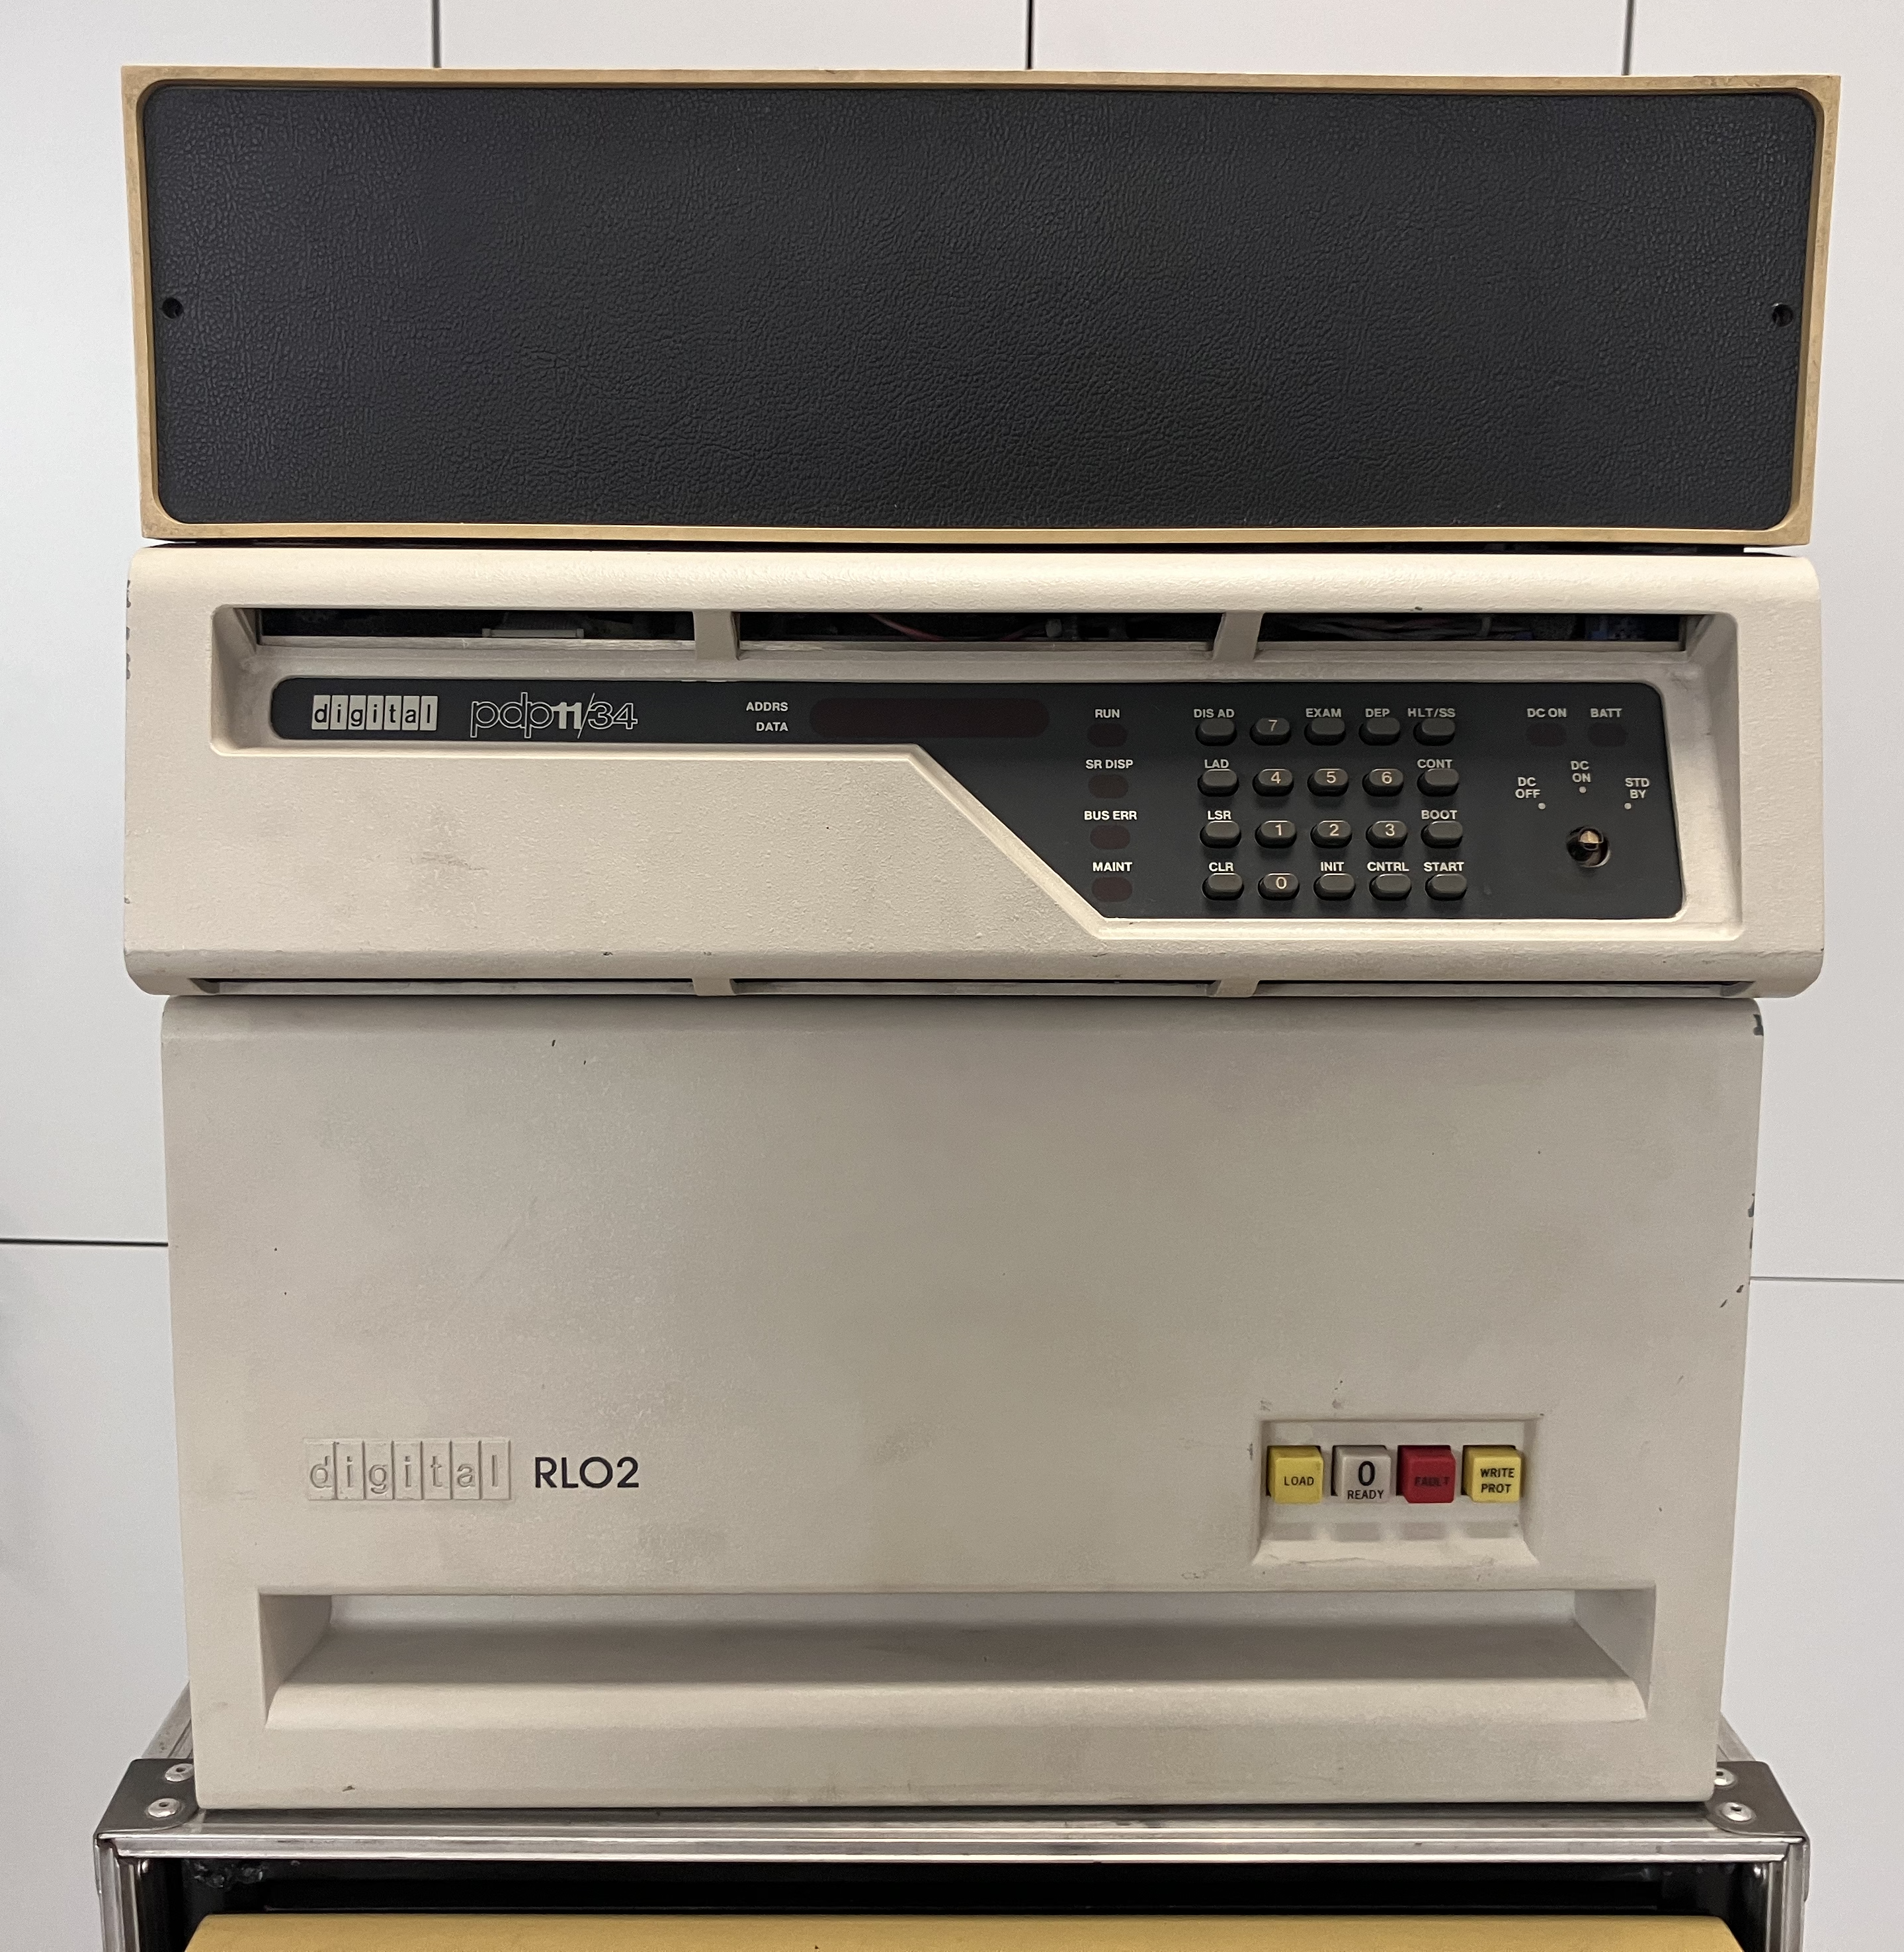
\includegraphics[width=0.7\linewidth]{chapters/appendix/c/image/figc-pdp11.png}
    \caption{PDP11/34 by Digital owned by Centro di Sonologia Computazionale (CSC) in Padua. This exact version was used to create all the \textit{Perseo e Andromeda}'s synthesis sounds. An earlier version was also used to create part of the Luigi Nono's Prometeo's sounds.}
    \label{fig:enter-label}
\end{figure}
All these pieces continue to be performed worldwide today, particularly Nono’s works, due to their significance and the scores that support them. These detailed scores have enabled the reuse of original devices and, over time, allowed for the adaptation of sound generation and processing techniques to new devices, thus supporting the ongoing technological migration of these works.

\section{\label{sec:ac-score-section}Score}
Table~\ref{tab:c-scores} provides some information about these scores.

\begin{longtable}{|p{0.3\textwidth}|p{0.1\textwidth}|p{0.1\textwidth}|p{0.3\textwidth}|p{0.2\textwidth}|}
    \caption{Scores (basic information)} \label{tab:c-scores} \\
    \hline
    \textbf{Piece} & \textbf{Premier} & \textbf{Score} & \textbf{Curated by} & \textbf{Edit by} \\
    \hline
    \scriptsize Das Atmende Klarsein \cite{nono1981das} & \scriptsize 1981 & \scriptsize (1st 1987) \textit{2005} & \scriptsize André Richard and Marco Mazzolini & \scriptsize Ricordi \\\hline
    \scriptsize Quando stanno morendo. Diario Polacco n.2 \cite{nono1982quando} & \scriptsize 1982 & \scriptsize (1st 1982) \textit{1999} & \scriptsize André Richard and Marco Mazzolini & \scriptsize Ricordi \\\hline
    \scriptsize Guai ai gelidi mostri \cite{nono1983guai} & \scriptsize 1983 & \scriptsize \textit{1983} & \scriptsize André Richard and Marco Mazzolini & \scriptsize Ricordi \\\hline
    \scriptsize A Pierre. Dell’azzurro silenzio inquietum \cite{nono1985a} & \scriptsize 1985 & \scriptsize (1st 1985) \textit{1996} & \scriptsize André Richard and Marco Mazzolini & \scriptsize Ricordi \\\hline
    \scriptsize Perseo e Andromeda \cite{sciarrino1990perseo} & \scriptsize 1990 & \scriptsize \textit{1992} & \scriptsize Salvatore Sciarrino, Alvise Vidolin, and Paolo Zavagna & \scriptsize Ricordi \\\hline
    \scriptsize Cantare con silenzio \cite{sciarrino1999cantare} & \scriptsize 1999 & \scriptsize \textit{1999} & \scriptsize Salvatore Sciarrino, Alvise Vidolin & \scriptsize Ricordi \\\hline
\end{longtable}

The first point to note is that many of these scores were published after the piece's premiere, even in the case of first editions. This fact suggests an ongoing refinement process following the first performance. Additionally, the editing of these scores is often carried out by collaborators rather than the composers themselves. For example, in the case of Nono, André Richard, the director of Freiburg’s Experimentalstudio, meticulously reissued Nono’s scores from the 1980s, clarifying the electronic parts. This reissuing, which took place after Nono died in the 1990s, included input from several of his collaborators.\\
For Sciarrino’s scores, we observe a similar approach: while Sciarrino himself handled the vocal and acoustic instrument parts, the electronic sections were developed with the assistance of Alvise Vidolin and, in the specific case of Perseo e Andromeda, also by Paolo Zavagna.\\
Another important factor in this study is that Ricordi, one of Italy’s leading music publishers, published all the scores, ensuring a consistent editorial approach across these works.\\
Considering the format of all these scores, we can see common sections, others less so, and differences in the order of appearance, naming and lexicon, but with the same or very similar purposes.\\
For all of these scores, we obviously have the \textit{temporal mapping}, i.e. the \textit{Score} in a traditional sense. The format of this section (the most extensive and important in a musical score) generally respects traditional musical notation, including non-standard and occasional modifications. For those pieces with singing parts (all the studied pieces except for \textit{A Pierre. Dell’azzurro silenzio inquitum}), the score also includes a \textit{Texts} section. Less common and less important from a technical perspective, there are sections such as the \textit{Index}, which helps navigate the document; \textit{Introduction}, which, when present, provides an abstract of the composition’s aesthetic and its connection to the text; and \textit{Notes} that offer details on how to interpret the score.\\
Other sections, almost always present, are \textit{Instrumentation}, which represents a list of all acoustic and electronic instruments used; \textit{Disposition}, which specifies the placement of acoustic instruments, the sound direction, performers, and speakers; \textit{Acoustic instruments instructions}, which provide information on non-standard notation and performance techniques for specific instruments; \textit{Electronic Instructions}, which outlines the electronic processes, setup requirements, and detailed performance instructions for the electronic elements across multiple pages; \textit{Schemas} which are related to the electronics instructions and give information the mappings of all the processes.\\
The Table~\ref{tab:c-score-sections} summarises the main sections commonly found in these scores. These sections are generalised since not all scores contain every section, and the terminology can vary.


\begin{longtable}{|p{0.14\textwidth}|p{0.14\textwidth}|p{0.14\textwidth}|p{0.14\textwidth}|p{0.14\textwidth}|p{0.14\textwidth}|p{0.14\textwidth}|}
    \caption{Scores sections} \label{tab:c-scores-sections} \\
    \hline
    \scriptsize\textbf{} & \scriptsize\textbf{Das Atemnde Klarsein} & \scriptsize\textbf{Diario Polacco n.2} & \scriptsize\textbf{Guai ai gelidi mostri} & \scriptsize\textbf{A Pierre} & \scriptsize\textbf{Perseo e Andromeda} & \scriptsize\textbf{Cantare con silenzio} \\
    \hline
    \scriptsize\textbf{Index} &  & \scriptsize p. V & \scriptsize Last page &  &  & \\\hline
    \scriptsize\textbf{Introduction} & & & \scriptsize pp. III-IV & & & \\\hline
    \scriptsize\textbf{Texts} & \scriptsize p. XXVII & \scriptsize p. LII & \scriptsize p. IV & & & \scriptsize p. I \\\hline
    \scriptsize\textbf{Instrumentation} & \scriptsize p. VI & \scriptsize p. VI &  & \scriptsize p. IV & &  \scriptsize p. II \\\hline
    \scriptsize\textbf{Disposition} & \scriptsize p. VI & \scriptsize p. VII & & \scriptsize p. IV & & \scriptsize p. 147 \\\hline
    \scriptsize\textbf{Acoustic instrument Instructions} & \scriptsize p. VII-X & \scriptsize pp. IX-XIV & \scriptsize pp. V-VII & \scriptsize pp. V-VII & & \scriptsize p. III \\\hline
    \scriptsize\textbf{Electronic instructions}	& \scriptsize pp. X-XII & \scriptsize pp.XXV-XXVIII	& \scriptsize pp. 94-96 & \scriptsize pp. VII-IX& \scriptsize pp. 123-125 & \scriptsize pp. 146-151 \\\hline
    \scriptsize\textbf{Schemas}	& \scriptsize pp. XXV-XXVI & \scriptsize pp. XLII-LI & \scriptsize pp. 106-111 & \scriptsize	p. IX & \scriptsize pp. 123-125 & \\\hline
    \scriptsize\textbf{Notes} & & & & \scriptsize p. X & \scriptsize p. 1 & \\\hline
    \scriptsize\textbf{Score} & \scriptsize pp. 1-22 & \scriptsize pp. 1-54 & \scriptsize pp. 1-74 & \scriptsize pp. 1-6 & \scriptsize pp. 1-121 & \scriptsize pp. 1-145 \\\hline
\end{longtable}
The \textit{Electronic Instructions} are essential to this study, as they have enabled and continue to allow the performance of these pieces despite the challenges of obsolescence and significant technological changes. The scores reference electronic devices not only on a surface level but also provide detailed descriptions that enable the original process to be recreated with different equipment based on the same principles. This adaptability is also supported by the widespread recognition of many of these processing tools. For instance, when the score mentions a ``harmonizer,'' there’s no need to explain how it works since this concept is well-understood in electronic music. However, in specific scores, such as \textit{Perseo e Andromeda}, the schematic description of an elementary synthesis (subtractive synthesis) is also included.\\
Some fundamental elements that we can find in the \textit{Electronic Instructions} section include (often as subsections):
\begin{itemize}
    \item \textit{Live Electronic Instruments List}: Often located in the \textit{Instrumentation} main section but sometimes specified within the \textit{Electronic Instructions} one (often with more detail). Here, we can find information on microphones, processors, speakers, mixers, and other equipment. This is shown in the score \textit{Guai ai gelidi mostri} and \textit{Cantare con silenzio}. In the latter, we see this subsection as a section per se and labelled as the tech rider.
    \item \textit{Microphone Setup}: Information on microphones, their placement, and routing. In live electroacoustic music, microphones are essential for capturing the live instrument sound, which is then processed. Although not always a separate section, this information is consistently included. For example, \textit{Cantare con silenzio} has an unconventional microphone setup with diagrams showing their placement (see Figure~\ref{fig:ac-microphones}). Sometimes, musicians and singers are given specific information on how to use the microphone. In \textit{Diario Polacco n.2}, specific microphone techniques for singers are indicated in the \textit{Acoustic Instrument Instructions} with original symbols, which are then used in the score.
    \item \textit{Disposition (Electronics)}: This section typically overlaps with the main section on \textit{Disposition} but provides more detailed information on the arrangement of equipment, particularly speaker placement (including height, distances, etc.).
    \item \textit{Processing and Parameters Description}: A key subsection in which each sound processing or generation process is described in detail. Descriptions are usually textual but may include graphics, diagrams, and charts. Each process also defines its parameters. In Nono’s scores, these details often reference devices from the Experimentalstudio. However, the descriptions focus less on specific devices and more on the underlying process. An example is the ``Reverser'' definition in \textit{Diario Polacco n.2}: ``\textit{The Reverser is an effect achieved with the Publison DHM 89 B2 in reverse mode. It has a memory duration of about 1.5 seconds, recording the signal in segments of 1.5 seconds in real-time while simultaneously replaying the previous segment in reverse}” \cite{nono1982quando}.
    \item \textit{Performance Instructions (Electronics)}: This subsection contains instructions on how to use electronics during the performance, often referencing non-standard symbols and notations in the score. This information is commonly found in Nono's scores and is usually labelled ``Dynamics,'' as live electronics often involve dynamic control of various processes during the performance. We also see the ``Program Transitions'' subsection (as in \textit{Guai ai gelidi mostri}), specifying how program (usually defined in the \textit{Schemas} section) changes and transitions should be managed in performance.
\end{itemize}

\begin{figure}[!h]
    \centering
    \includegraphics[width=0.8\linewidth]{chapters/appendix/c/image/figc-microphones.png}
    \caption{The microphone placement (M1, M2, and M3 are the microphones) in the tam-tam, large bell plate (Campana Lastra), and metal sheet (Lastra) in \textit{Cantare con silenzio}.}
    \label{fig:ac-microphones}
\end{figure}

Another important section is the \textit{Schemas}, which, although often separated from the \textit{Electronic Instructions}, is closely related to it. Here, various processes for sound processing or generation are described across different levels of detail.\\
In some cases, the processes are explained at a basic level, describing sound processing or synthesis from fundamental elements. For example, in \textit{Perseo e Andromeda}, the schemas provide definitions for subtractive synthesis: how the basic element of noise is linked to the filters and how they are modified through basic parameters (volume, resonance factor, central frequency). Two different schema types are shown: a general description (Figure~\ref{fig:ac-perseo-schema01}) and a more specific one for describing the implementation in Music5, the programming language used in the original composition (Figure~\ref{fig:ac-perseo-schema01}).

\begin{figure}[!h]
    \centering
    \includegraphics[width=\linewidth]{chapters/appendix/c/image/figc-perseo-schema01.png}
    \caption{High-level schema used in \textit{Perseo e Andromeda}’s score to describe the subtractive synthesis.}
    \label{fig:ac-perseo-schema01}
\end{figure}

\begin{figure}[!h]
    \centering
    \includegraphics[width=\linewidth]{chapters/appendix/c/image/figc-perseo-schema02.png}
    \caption{The schema used in \textit{Perseo and Andromeda}’s score describes the subtractive synthesis according to the Music5 programming language.}
    \label{fig:ac-perseo-schema02}
\end{figure}

Alternatively, some schemas offer a higher-level view, showing signal routing and how different devices and processing systems communicate. These schemas are often used in Nono's scores, defining processing programs for performance. In \textit{Diario Polacco n.2}, for example, \textit{Program 11} (Figure~\ref{fig:ac-nono-schema01}) illustrates signal routing, showing how microphone signals pass through various processors (described in the \textit{Processing and Parameters Description} subsection) and ultimately reach the speakers.

\begin{figure}[!h]
    \centering
    \includegraphics[width=\linewidth]{chapters/appendix/c/image/figc-nono-schema01.png}
    \caption{\textit{Diario Polacco n.2}'s \textit{Program 11}’s signal routing and processing communication.}
    \label{fig:ac-nono-schema01}
\end{figure}

The \textit{Perseo e Andromeda} score also includes a top-level schema that maps the physical connections (\textit{physical implementation mapping}) between devices like computers, mixers, and controllers rather than just logical connections or signal routing (Figure~\ref{fig:ac-perseo-schema03}).

\begin{figure}[!h]
    \centering
    \includegraphics[width=0.8\linewidth]{chapters/appendix/c/image/figc-perseo-schema03.png}
    \caption{The \textit{Perseo e Andromeda}’s \textit{physical implementation mapping} between computers, mixer and controllers.}
    \label{fig:ac-perseo-schema03}
\end{figure}

Though these schemas vary in detail and purpose across different scores, they all employ a block diagram format, a design approach borrowed from electrical circuit schematics and diagrams.\\
These are the main elements shared across the various scores. Beyond these, each score includes unique or specific elements, often required for implementing particular aspects of a composition or, at times, added to enrich the information available for performance. For example, \textit{Perseo e Andromeda} includes an additional 88 pages at the end of the score, containing the complete source code of the composition written in Music5 (Figure~\ref{fig:ac-perseo-code} shows the first page of this source code).

\begin{figure}[!h]
    \centering
    \includegraphics[width=0.8\linewidth]{chapters/appendix/c/image/figc-perseo-code.png}
    \caption{First page of the 88 pages of the source code in Music5 for the \textit{Perseo e Andromeda} live electronics performance.}
    \label{fig:ac-perseo-code}
\end{figure}

\section{Reactivation}
All the pieces mentioned here were reactivated as part of the research project to study the use of scores in performance settings. Five of these works — all of Nono's compositions and \textit{Cantare con silenzio} by Sciarrino — were reactivated in the context of the \textit{Live Electronics Sound and Music Computing} course at the Chigiana Summer Academy in the summer of 2022. This month-long course, which takes place each summer, is led by Alvise Vidolin and Nicola Bernardini and focuses on studying live electronics pieces and their performance.\\
The courses focused on understanding, using and reactivating all real-time sound processing or synthesis systems, studying analogue and digital devices, and adapting or migrating them to current technologies. For the performances of Nono's works and Sciarrino's \textit{Cantare con silenzio}, all sound processing techniques were recreated under the teachers' guidance, using Max/MSP, a Visual Programming Language (VPL) widespread in live electronics performance (and increasingly for multimedia arts). These five pieces were performed in four concerts as part of Chigiana's 2022 summer concert series, dedicated to Luigi Nono and titled \textit{From Silence}.

\begin{itemize}
    \item \textit{Luigi Nono. Un silenzio inquieto (I)} (July 14, 2022). Among the performed pieces, the concert also included \textit{Quando stanno morendo. Diario polacco n. 2} and \textit{Luigi Nono A Pierre. Dell’azzurro silenzio}. The event link: \url{https://www.chigiana.org/pf/14-luglio-2022/}.
    \item \textit{Luigi Nono. Un silenzio inquieto (III)} (July 19, 2022). Among the performed pieces, the concert included \textit{Das atmende Klarsein}. TThe event link: \url{https://www.chigiana.org/pf/19-luglio-2022-2/}.
    \item \textit{Luigi Nono. Un silenzio inquieto (IV)} (July 22, 2022). Among the performed pieces, the concert included \textit{Guai ai gelidi mostri}. The event link: \url{https://www.chigiana.org/pf/22-luglio-2022/}.
    \item \textit{Luigi Nono. Un silenzio inquieto (V)} (July 27, 2022). Among the performed pieces, the concert included \textit{Cantare con silenzio}. The event link: \url{https://www.chigiana.org/pf/27-luglio-2022/}
\end{itemize}
The opera \textit{Perseo e Andromeda} was reactivated and performed independently, outside the context of the Chigiana Academy. This case provided an opportunity to independently study the use of the score in reactivating and performing the piece, applying the teachings from the Chigiana course while also testing the MDC model and CATTA workflow developed during the thesis project.\\
\newline
The city of Rimini promoted the performance of \textit{Perseo e Andromeda} as part of the 74th edition of the \textit{Sagra Musicale Malatestiana} (2023), one of Italy’s oldest and most renowned music festivals. The direction was entrusted to artists Daniele Spanò and Luca Brinchi, known for their experimental theatre and multimedia artwork, who reimagined Sciarrino’s piece as a complete multimedia installation. At the initiative of the festival’s artistic direction, the musical performance was assigned not to the historical performers but to emerging talents: Eleonora Benetti (Andromeda), Arianna Lanci (Dragon), Giacomo Pieracci and Paolo Leonardi (Perseus), and Mattia Dattolo (Conductor)\footnote{However, the new performers received special help and support from the historical performers, especially Alda Caiello (for the vocal part) and Alvise Vidolin (for the electronic part).}.\\
The following section will summarise the entire process of reactivating the piece according to the CATTA reactivation workflow.

\subsection*{Collection}
\textit{Perseo e Andromeda} has performed only four times: the premiere in 1991 (Staatstheater, Stuttgart), twice in 1992 (at \textit{Festival Orestiadi} in Gibellina and Teatro Lirico in Milan), and once in a non-staged version in 2000 (\textit{Festival d’Automne} in Paris). In addition to these performances, an audio recording session for a CD of the opera was held in 2000.\\
The case study began by gathering documentation on the opera (the score and technical instructions) and its various performances. Limited photographic and video documentation of individual performances was available. Additionally, pieces of code and software (Max/MSP) used in the 2000 performances were collected.\\
Crucial information was provided by oral histories of technicians and performers in past productions—especially Alvise Vidolin and soprano Alda Caiello—as well as insights from the composer himself. This collection was then organised according to the MDC model.

\subsection*{Assessment}
During the documentation evaluation, the performance scores and technical instructions were carefully analysed. Additionally, by reviewing the performance history, previous technological migrations were identified, especially regarding the main computer:
\begin{itemize}
    \item 1991: PDP11 computer with 4i audio processor;
    \item 1992: IRIS SM1000 (MARS) system;
    \item 2000: Apple computer (undefined model) using Max/MSP environment.
\end{itemize}
After assessing reactivation options, the restoration of the PDP11/34 computer and IRIS SM1000 system was ruled out due to their obsolescence and complexity (despite recent restorations at the CSC). The 2000 Max/MSP environment was tested, and issues related to reactivation were identified.\\
The design space was defined by starting with the Max/MSP 2000 environment, identifying development paths to upgrade the system with new computers, updated Max/MSP versions, and modern I/O communication protocols.

\subsection*{Transcription}
Following the development paths and the score, we introduced upgrades to the Max/MSP software, which modernised the execution environment and addressed previous issues. This Max/MSP update required an upgrade in hardware, including new performance management systems and updated audio routing protocols (Dante).\\
Developing the new execution environment required revisiting the prototyping phase several times to optimise parts of the software.

\subsection*{Transmission}
The performance environment was developed before and during a long rehearsal session held in October 2023. During this time, the setup and the performance were adapted to meet the needs of the director, singers, and conductor. Thanks to streamlining and advancements in new technology, this performance became the first in the history of \textit{Perseo e Andromeda} to be executed by a single live electronics operator.\\
The performance of \textit{Perseo e Andromeda} took place on October 20, 2023, at the Teatro degli Atti in Rimini. Figure~\ref{fig:ac-perseo-ph03}, Y, Z, and U are photos from the event, providing a glimpse into the visionary direction by Daniele Spanò and Luca Brinchi.

\begin{figure}[!h]
    \centering
    \includegraphics[width=\linewidth]{chapters/appendix/c/image/figc-perseo-ph003.jpg}
    \caption{Photos of the performance of \textit{Perseo e Andromeda} in Rimini on 20 October 2023.}
    \label{fig:ac-perseo-ph03}
\end{figure}

\subsection*{Archiving}
The \textit{Transcription} phase was thoroughly documented, with specific instructions for setting up the updated system (see stage plan or spatial mapping in Figure~\ref{fig:ac-mapping-spatial} and physical implementation Figure~\ref{fig:ac-mapping-physical}). The transmission phase was captured through photos in Figure~\ref{fig:ac-perseo-ph01}, \ref{fig:ac-perseo-ph02}, and \ref{fig:ac-perseo-ph03}, audio, and video recordings of the dress rehearsal and final performance. Additionally, \textit{Sagra Malatestiana} produced a documentary.\\
All documentation was archived using the MDC model. Unlike other case studies—where tools like Neo4j were used for \textit{videoloop} (Appendix~\ref{ax:a-michele_sambin_videoloop}) and \textit{Il caos delle sfere} (Appendix~\ref{ax:b-hybrid_reactivation_il_caos_delle_sfere}), or GitHub for Soundrise and Cadavid’s instruments (Appendix~\ref{ax:d-sustainability_and_longevity_of_nimes})—this example applied the MDC model to organise a local folder on a computer using the macOS system. This approach was chosen because various institutions already manage and archive the compositions studied here. For Nono, the score is managed by Ricordi and archived by Fondazione Archivio Luigi Nono ONLUS; for Sciarrino, the scores are also managed by Ricordi (with a new version completed in 2023) and archived by both the Ricordi Historical Archive and the Paul Sacher. However, these institutions don’t yet fully handle the electronic components (beyond documentation in the score)\footnote{Actually, the latest version of the score for \textit{Perseo e Andromeda} includes software and sound files necessary for the performance (though not comprehensive). Unfortunately, these were not used during the reactivation process as they were published and delivered only a few weeks before the performance.}. Furthermore, due to copyright restrictions, publishing an implementation (\textit{Transcription}) of these pieces within a separate repository or archive is impossible. This case, therefore, represents a personal archive (or a ``actor archive'') used to track the development stages of a project with essential tools such as personal computer folders. Chapter~\ref{ch:4-madc_model_application} explores the application of the MDC model using the file management system Finder for creating an ``actor archive.''

\section{Data compilation}
As with the \textit{videoloop} described in Appendix~\ref{ax:a-michele_sambin_videoloop}, the setup and technical preparation of the entire artwork also required the help and work of technicians. Again, we needed to create a tech rider—something not included in the score—to coordinate the setup. Below, we provide the \textit{List of bits and specifications}, the \textit{stage plan} (or \textit{spatial mapping}), and the physical implementation mapping as they appear in the tech rider. In this case, The tech rider comprehends only the audio specifications.

\subsection*{List of bits and specifictions}
Table~\ref{tab:c-data-bits} reports the list of bits divided by hardware and software with the related specifications and requirements.
\begin{longtable}{|p{0.3\textwidth}|p{0.05\textwidth}|p{0.55\textwidth}|}
    \caption{Hardware} \label{tab:c-data-bits} \\
    \hline
    \textbf{Name} & \textbf{Q} & \textbf{Specification and notes} \\
    \hline
    Full range speakers & 12 & \scriptsize (S1, S2) \textbf{HORIZON} (H) Placed at the back of the stage; (S3, S4) \textbf{FRONT/SPREAD} (F) Placed in front of the stage. Height $\sim$250/300 cm above the floor; (S5, S6) \textbf{UPPER} (T) Placed in the ceiling, above and facing the audience; (S7, S8) \textbf{BACK} (R) Placed at the back of the hall (last seats). Height $\sim$250/300 cm from the floor; (S9, S10, S11, S12) \textbf{DIFFUSION} (R) Placed around the audience. Height $\sim$200/300 cm from the floor\\\hline
    Subwoofer & 2 & \\\hline
    Digital Mixer & 1 & \scriptsize $\geq$4 analog in; $\geq$16 analog out; 16 in x16 out Dante.\\\hline
    Radio microphone & 4 & \scriptsize Miniature Omnidirectional microphone e.g. DPA 4060 \\\hline
    Laptop & 1 & \scriptsize Apple Macbook Pro (Silicon) macOS (14.1.2); Max/MSP (8.5.6); Dante Virtual Sound Card (4.4.1.3).\\\hline
    Controller MIDI & 1 & \scriptsize 8 Motorised Fader USB. \textbf{Suggested}: BEHRINGER x-touch Extender.\\\hline 
    Launchpad MIDI & 1 & \scriptsize 16 pads USB. \textbf{Suggested}: AKAI MPD 218. \\\hline 
\end{longtable}

\begin{longtable}{|p{0.35\textwidth}|p{0.55\textwidth}|}
    \caption{SOFTWARE} \label{tab:c-data-bits} \\
    \hline
    \textbf{Name} & \textbf{Specification and notes} \\
    \hline
    Max/MSP & \scriptsize version 8.5.6. \\\hline
    Dante Virtual Sound Card & \scriptsize version 4.4.1.3 \\\hline
    Perseo e Andromeda Max/MSP Patch & \scriptsize 2023 version Performance patch \\\hline 
\end{longtable}

\subsection*{Spatial mapping}
Figure~\ref{fig:ac-mapping-spatial} shows the stage plan of the Perseo and Andromeda, as reported in the tech rider. 

\subsection*{Physical implementation}
Figure~\ref{fig:ac-mapping-physical} shows a physical implementation of the opera \textit{Perseo e Andromeda} using the BVL. This mapping shows how the individual \textit{bit}s should be linked together and interact between them. 

\begin{figure}[!h]
    \centering
    \includegraphics[width=0.8\linewidth]{chapters/appendix/c/image/graphc-mapping-physical.png}
    \caption{\textit{Physical implementation mapping} of \textit{Perseo e Andromeda}. Link and interaction between \textit{bit}s.}
    \label{fig:ac-mapping-physical}
\end{figure}

\section{Results and discussion}
The use of scores in live electronics music is essential and almost always outweighs the importance of specific devices. As we’ve seen with \textit{Perseo e Andromeda} and other works, scores not only allow us to reconstruct all signal processing and generation systems independently of the technology used, but they also ensure the work's longevity through potential future technology migrations. This approach supports the concept of ``medium independence,'' which has been highlighted since the late 1990s in the conservation of live media art. It is no coincidence that many scholars, artists and conservators in this field compare live media art with music, emphasising the importance of scores.\\
Another relevant case study not discussed in this thesis is \textit{Lamento} (2007) for voice and live electronics by the French composer Franck Bedrossian. This piece, created in collaboration with IRCAM in Paris, currently exists only as a handwritten score that lacks electronic instructions for implementation and performance, making it heavily dependent on the IRCAM software used to produce it. Outside this doctoral project but still relevant, \textit{Lamento} was performed twice—first in 2022 at a Divertimento Ensemble concert in Milan and again in 2024 at the 2nd \textit{Sacred Music Festival} by the Greek National Opera in Athens. In both cases, technical issues arose with the IRCAM software. In the first instance, the composer provided an outdated software version, requiring a 2014 computer (since the libraries were incompatible with newer systems). In the second, IRCAM supplied an updated version of the code that still needed some revisions for practical use. This piece exemplifies a closed system without documentation, where the only source of information is the code itself, which must be painstakingly examined to understand processes and fix errors or compatibility issues. Due to the lack of a score, this piece will always be tied to IRCAM or, more specifically, to the original technicians who developed the software, requiring periodic updates and a transmission of knowledge, either documented or verbal, related to the composition and its electronics. While the electronics for \textit{Lamento} may not be entirely lost without a score, their reactivation will become increasingly complex over time\footnote{It's important to emphasize that the absence of the score is not the fault of either the composer or IRCAM. Indeed, I would like to express my gratitude to IRCAM, especially to Serge Lemouton and Cyril Béros, who provided valuable support and assistance in implementing the live electronics for Franck Bedrossian’s Lamento.}.\\
These case studies highlight the importance of scores in conserving and transmitting artworks, whether a live electronics piece or a live media art installation or performance. However, one of the main arguments of this text is that there is no standard formats and lexicon for creating scores in electronic music, let alone in live media art. In light of the models and visual language covered in Chapter~\ref{ch:3-mdc_model-reactivation_workflow-instruction_template}, it’s clear that a standard language may not be feasible, and documentation practices may need to remain open and flexible. Nevertheless, Chapter~\ref{ch:3-mdc_model-reactivation_workflow-instruction_template} introduced an instruction template based on the live electronics scores studied above. We introduced Baalman’s visual language (BVL) within the template as guidelines to describe the processes and implementation of artworks. The introduction of the BVL does not mean it verbatim but rather as an example for creating a customised language suited to each unique work. This language, which in this thesis has been slightly remodelled (in Chapter~\ref{ch:4-madc_model_application}), generally follows the format of circuit descriptions found in electronic music scores and extends to various types of art with different levels of detail and information. Thus, we can see the BVL as a flexible guideline for describing any kind of live media art (also comprehending music), adaptable to specific descriptive needs. Figure~\ref{fig:ac-mapping-physical}, for example, redefines the \textit{physical implementation mapping} through the BVL based on the new technologies used in \textit{Perseo e Andromeda} and can be compared with the initial \textit{physical implementation mapping} outlined in Figure~\ref{fig:ac-perseo-schema03} in the original score and designed by Alvise Vidolin and Paolo Zavagna.\\

\begin{figure}[!h]
    \includegraphics[width=\linewidth]{chapters/appendix/c/image/graphc-mdc.png}
    \caption{Approximate chronological representation of \textit{Perseo e Andromeda} according to the MDC model.}
    \label{fig:ac-graph_mdc}
\end{figure}

Figure~\ref{fig:ac-graph_mdc} shows an approximate representation of \textit{Perseo e Andromeda} through the MDC Model.


\begin{figure}
    \centering
    \includegraphics[width=\linewidth]{chapters/appendix/c/image/graphc-mapping-spatial.png}
    \caption{Stage plan (\textit{spatial mapping}) of \textit{Perseo e Andromeda} opera.}
    \label{fig:ac-mapping-spatial}
\end{figure}